\begin{figure}[!htbp]
    \centering
    \begin{subfigure}[b]{0.8\textwidth}
        \centering
        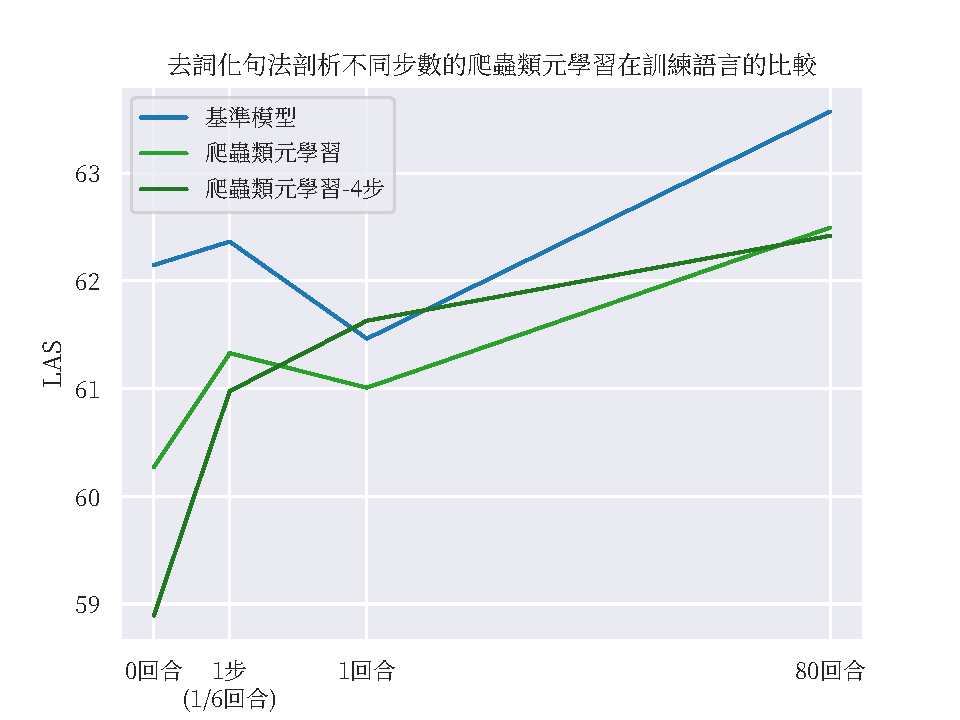
\includegraphics[width=\textwidth]{figs/chapter3/delex/delex_reptile_train_langs.pdf}
    \end{subfigure}
    \vspace{-12pt}
    \begin{subfigure}[b]{0.8\textwidth}
        \centering
        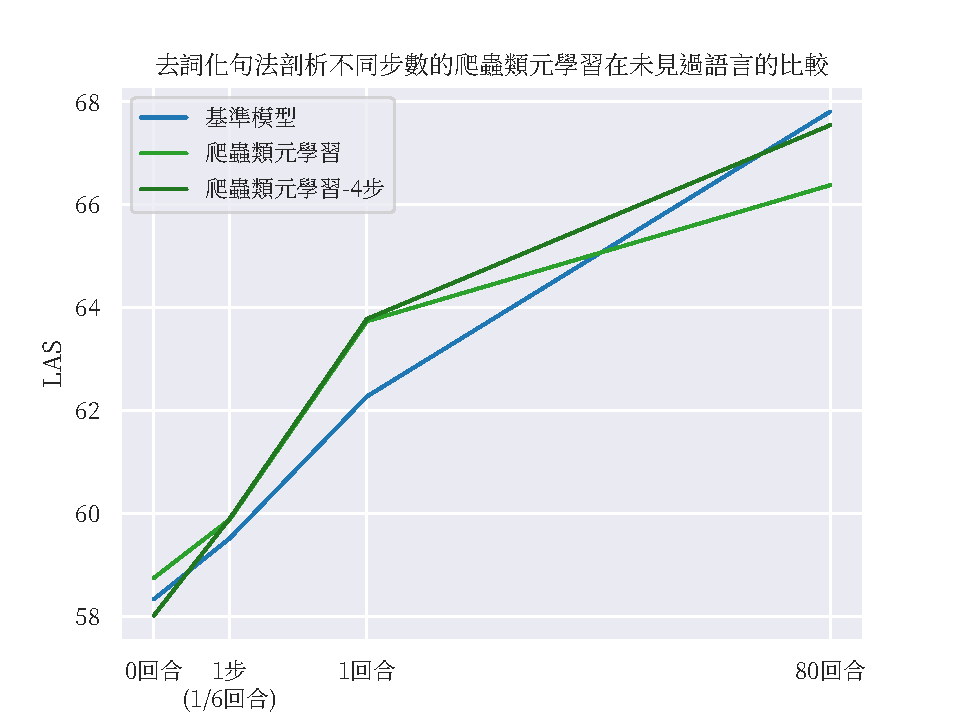
\includegraphics[width=\textwidth]{figs/chapter3/delex/delex_reptile_test_langs.pdf}
    \end{subfigure}
    \caption{去詞化分析不同步數的爬蟲類元學習精細校正後在測試集上的平均表現。}
    \label{fig:delex_avg}
\end{figure}